% !TEX TS-program = lualatex
% !TEX encoding = UTF-8 Unicode

\documentclass[professionalfonts]{beamer}
\usepackage{iftex,ifxetex}
\ifPDFTeX
  \usepackage[utf8]{inputenc}
  \usepackage[T1]{fontenc}
  \usepackage{lmodern}
\else
  \ifluatex
    \usepackage{unicode-math} 
    \defaultfontfeatures{Ligatures=TeX}
    % \setmathfont{Latin Modern Math}
    \setsansfont{CMU Sans Serif}
    % \setsansfont{Linux Biolinum O}
  \fi
\fi

\mode<presentation>
{
  \usetheme{Madrid} % or try Darmstadt, Madrid, Warsaw, ...
  % or ...
  \setbeamertemplate{bibliography item}{}
  \setbeamercovered{transparent}
  % or whatever (possibly just delete it)
}

\usepackage{fontspec}
\usepackage[english]{babel}
% or whatever
\usepackage{csquotes}
\usepackage[backend=biber,
        style=unified,
        maxcitenames=3,
        maxbibnames=99,
        natbib,
        url=false]{biblatex}
% \addbibresource{Dissertation.bib}
\setmainfont{Libertinus Sans} % Main font
% \setsansfont{libertinus sansserif} % Sans serif font
% \setmonofont{CMU Typewriter Text}
\renewcommand{\ttdefault}{cmtt}

% \usepackage[colorlinks,allcolors={black},urlcolor={blue}]{hyperref} %allows for hyperlinks and pdf bookmarks 
\usepackage{graphicx}	%Inserting graphics, pictures, images 		
\usepackage{multicol} %Multicolumn text
\usepackage{multirow} %Useful for combining cells in tablesbrew 
% \usepackage{booktabs} %Enhanced tables
% \usepackage{underscore} %Allows for underscores in text mode
% \usepackage[colorlinks,allcolors={black},urlcolor={blue}]{hyperref} %allows for hyperlinks and pdf bookmarks
\usepackage{url} %allows for urls
\def\UrlBreaks{\do\/\do-} %allows for urls to be broken up
% \usepackage[normalem]{ulem} %strike out text. Handy for syntax
% \usepackage{tcolorbox}
% \usepackage{datetime2}
\usepackage{caption}
\usepackage{subcaption}
\usepackage{langsci-gb4e} % Language Science Press' modification of gb4e
\usepackage{tikz} % Drawing Hasse diagrams
\usetikzlibrary{decorations.pathreplacing}
\usepackage{leipzig} %	Offers support for Leipzig Glossing Rules
% \usepackage{animate} % For creating animations in PDF slides
\usepackage{annotate-equations}

% Hyperlink settings
\hypersetup{
    colorlinks,
    urlcolor=blue,        % Color for URLs
    linkcolor=white        % Color for internal links
}

\title[LING 450/550] % (optional, use only with long paper titles)
{Introduction to Linguistic Phonetics}

\subtitle{Acoustics of Vocoids}

\author[Brinkerhoff] % (optional, use only with lots of authors)
{Mykel Loren Brinkerhoff}
% - Give the names in the same order as the appear in the paper.
% - Use the \inst{?} command only if the authors have different
%   affiliation.

\institute[UW] % (optional, but mostly needed)
{University of Washington}
% - Use the \inst command only if there are several affiliations.

\date[2025-10-16] % (optional, should be abbreviation of conference name)
{October 16, 2025}

% If you have a file called "university-logo-filename.xxx", where xxx
% is a graphic format that can be processed by latex or pdflatex,
% resp., then you can add a logo as follows:

% \pgfdeclareimage[height=0.5cm]{university-logo}{university-logo-filename}
% \logo{\pgfuseimage{university-logo}}



% Delete this, if you do not want the table of contents to pop up at
% the beginning of each subsection:
% \AtBeginSubsection[]
% {
%   \begin{frame}<beamer>{Outline}
%     \tableofcontents[currentsection,currentsubsection]
%   \end{frame}
% }


% If you wish to uncover everything in a step-wise fashion, uncomment
% the following command: 

%\beamerdefaultoverlayspecification{<+->}


\begin{document}

\begin{frame}
    \titlepage
\end{frame}

%-----------------------------------------------------------
\section{Introduction}
%-----------------------------------------------------------

% \begin{frame}{Which medieval cat are you?}
    
%     \begin{center}
%         \includegraphics[width = .5\linewidth]{figs/MedievalCatIcebreaker.jpeg}
%         \url{https://pollev.com/mykellorenbrinkerhoff821} or text/SMS mykellorenbrinkerhoff821 to 22333
%     \end{center}
% \end{frame}

\begin{frame}{Reflections}
    \begin{block}{Reflection}
        \begin{itemize}
            \item Spend $\thicksim$3 minutes reviewing your notes from last lecture, homeworks, exit tickets, etc.
            \item Look for questions you have or clarifications you would like. 
        \end{itemize}
    \end{block}
\end{frame}

\begin{frame}{Recap from last time}
    \begin{itemize}
        \item The glottis produces sound (the source and correlated with \textit{f0}) which resonates in the vocal tract (the filter) 
        \item Changing the position of the articulators changes the resonances by making constrictions at nodes and anti-nodes (perturbation)
        \item We can see resonances on a spectrum as peaks of high energy in harmonics, and on a spectrogram as dark horizontal bands
        \item These areas of resonance are called formants
    \end{itemize}
\end{frame}

\begin{frame}{Size matters}
    \begin{center}
        \href{https://youtu.be/lebTZB0pELc}{\includegraphics[width=\linewidth]{figs/Recorders.jpg}}
    \end{center}
\end{frame}



%-----------------------------------------------------------
\section{Vowels}
%-----------------------------------------------------------

\begin{frame}{Vowels}
    \begin{itemize}
        \item Vowels have relatively wide open vocal tract
        \item This means they are relatively loud and have clear, easy to identify resonances
        \item The vocal folds provide the source of sound / energy
        \item The position of the tongue determines the resonances, along with the lips
    \end{itemize}
\end{frame}

\begin{frame}{Some things to remember}
    \begin{itemize}
        \item The longer the tube, the lower the resonances
        \item A constriction at a pressure node (particle movement antinode) lowers resonances
        \item A constriction at a pressure anti-node (particle movement node) raises resonances
        \item There are multiple resonances for any given configuration of the vocal tract 
        \begin{itemize}
            \item (i.e., there are theoretically an infinite number of formants)
        \end{itemize}
        \item The vocal folds provide energy at a range of frequencies to resonate in the vocal tract
    \end{itemize}
\end{frame}

\begin{frame}{Formants}
    \begin{itemize}
        \item Formants are what we call the vocal tract resonances
        \item We see them as peaks in a spectrum and dark horizontal bands in a spectrogram
        \item We primarily rely on the first three vocal tract resonances to define different vowels (with the first two being the most crucial)
    \end{itemize}
\end{frame}

\begin{frame}{Formants}
    \begin{center}
        \includegraphics[width=\textwidth]{figs/rj-c10f002.jpg}
    \end{center}
\end{frame}

\begin{frame}{Formants}
    \begin{center}
        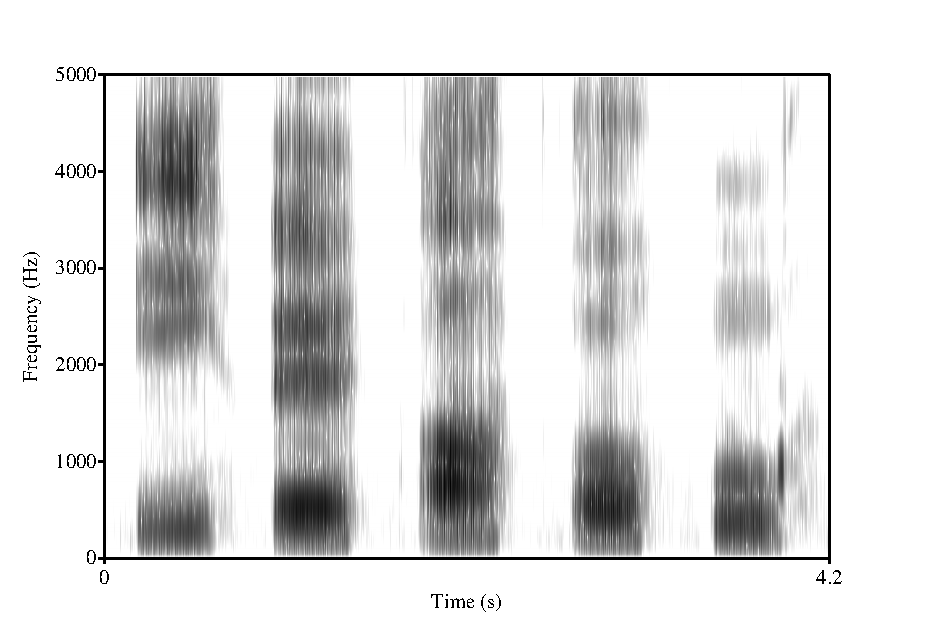
\includegraphics[width=\linewidth]{figs/mlb_ieaou.eps}
    \end{center}
\end{frame}

\begin{frame}{First Formant (F1)}
    \begin{itemize}
        \item In adults, it varies from about 200Hz to 800Hz
        \item Opening the lips and lowering the jaw / tongue will raise it
        \item Essentially, vowel “height” is inversely related to the first formant (F1)
        \item Example: /i/ has a lower F1 than /a/
    \end{itemize}
\end{frame}

\begin{frame}{Second Formant (F2)}
    \begin{itemize}
        \item The second formant ranges from 700 Hz to 2400Hz in adults
        \item It can be raised by moving the tongue forward
        \item Thus, it generally correlates with backness
        \begin{itemize}
            \item The “fronter” the vowel, the higher the F2
            \item So /i/ has a higher F2 than /u/
        \end{itemize}
        \item For the high vowels, F2 generally derives from the front cavity resonances
        \begin{itemize}
            \item Note that rounding will lower the front cavity resonance by both lengthening the vocal tract ahead of the constriction and forming a helmholtz resonator\footnote{A closed off chamber that can resonant}
        \end{itemize} 
    \end{itemize}
\end{frame}

\begin{frame}{F1xF2}
    \begin{center}
        \includegraphics[width=\linewidth]{figs/rj-c10f001.jpeg}
    \end{center}
\end{frame}


\begin{frame}{Third Formant (F3)}
    \begin{itemize}
        \item The third vocal tract resonance varies from 2000Hz 3000Hz
        \item \textbf{It is not nearly as neatly aligned with the articulatory features of vowels!}
        \begin{itemize}
            \item That is, it’s not as important for defining front / back distinctions
        \end{itemize}
        \item English /ɚ,ɹ/ generally have a low F3
        \item Front round / unround pairs \textit{sometimes} show F3 differences
        \begin{itemize}
            \item In these cases, front round vowels usually have an F3 lowered to near F2
        \end{itemize}
        \item But rounding also affects F1 and F2!
    \end{itemize}
\end{frame}

\begin{frame}{Formant lowering}
    \begin{center}
        \includegraphics[width=\linewidth]{figs/rj-c10f003.jpeg}
    \end{center}
\end{frame}

\begin{frame}{The vowel trapezoid}
    \begin{block}{Question:}
        What does this have to do with our vowel trapezoid?
    \end{block}
    \begin{center}
        \includegraphics[width=0.75\linewidth]{figs/IPAVowels.png}
    \end{center}
\end{frame}

\begin{frame}{The F1-F2 plane}
    \includegraphics[width = \linewidth]{figs/F1xF2.jpg}
\end{frame}

%-----------------------------------------------------------
\section*{Break}
%-----------------------------------------------------------

\begin{frame}{Break Time!}
    \begin{center}
        \Huge 10 minute break \\ (stretch, grab a drink, etc.)
    \end{center}
\end{frame}

%-----------------------------------------------------------
\section*{Glides}
%-----------------------------------------------------------

\begin{frame}{Approximants}
    \begin{itemize}
        \item Approximants are acoustically very similar to vowels. 
        \item However, there is not a really good definition for what an approximant is. 
        \item Essentially, they are a sound that is somewhere between a vowel and consonant 
        \begin{itemize}
            \item This is why they are sometimes called \textit{semivowels}
        \end{itemize}
        \item This term is what we technically call a ``trashcan''-term\footnote{Credit to Ryan Bennett (UCSC).}
    \end{itemize}
\end{frame}

\begin{frame}{Approximants}
    \begin{center}
        \includegraphics[width = \textwidth]{figs/padgett-2008.jpg}
    \end{center}
\end{frame}

\begin{frame}{Approximants}
    \begin{center}
        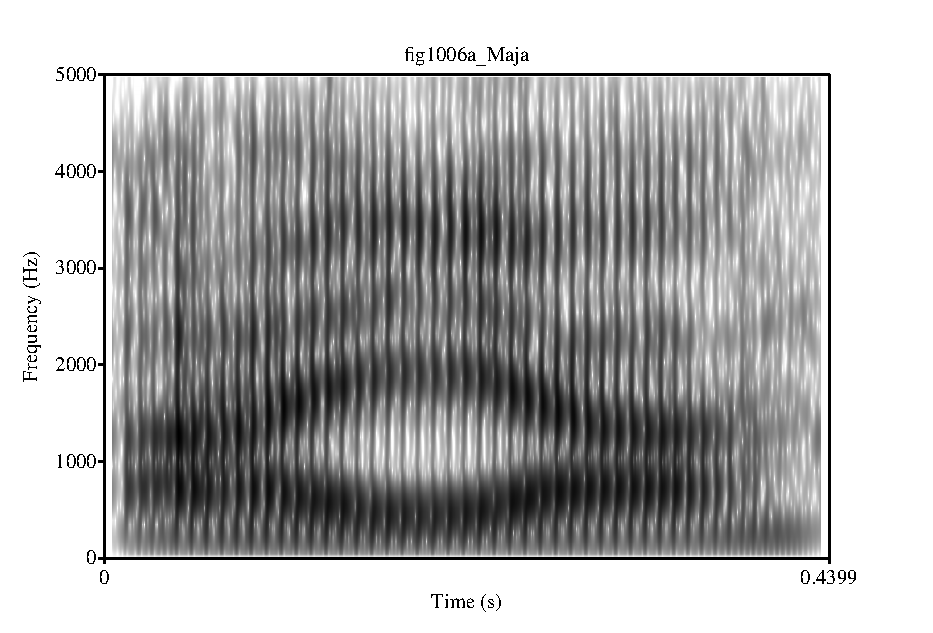
\includegraphics[width = \textwidth]{figs/aja.eps}
    \end{center}
\end{frame}

\begin{frame}{Approximants}
    \begin{center}
        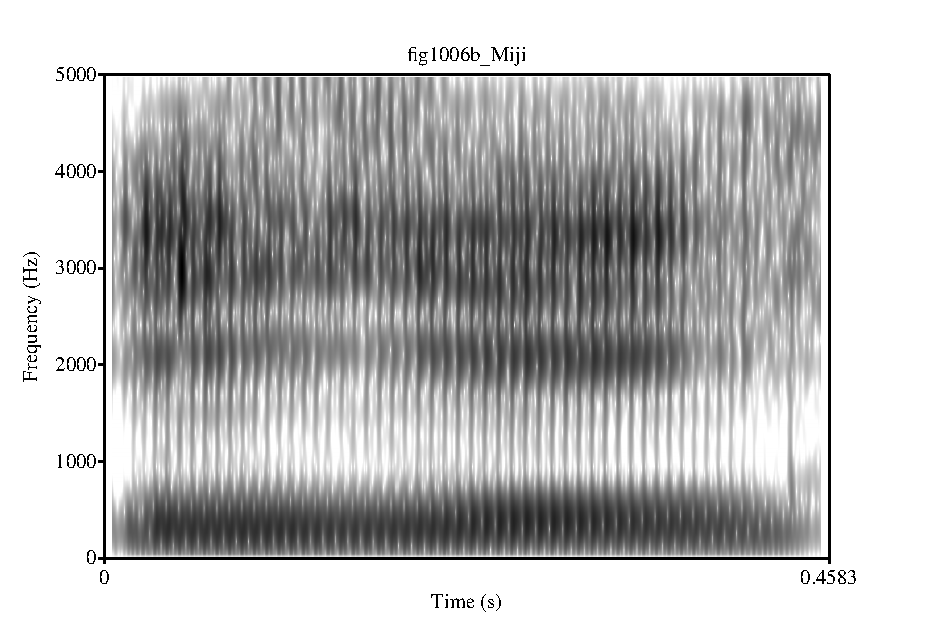
\includegraphics[width = \textwidth]{figs/iji.eps}
    \end{center}
\end{frame}

\begin{frame}{Approximants}
    \begin{center}
        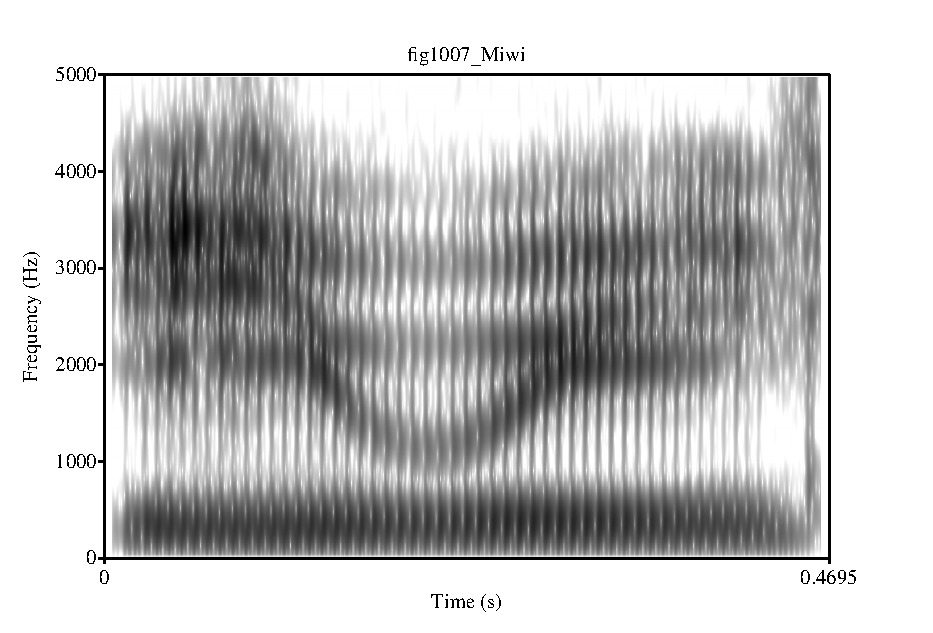
\includegraphics[width = \textwidth]{figs/iwi.eps}
    \end{center}
\end{frame}

\begin{frame}{Approximants}
    \begin{center}
        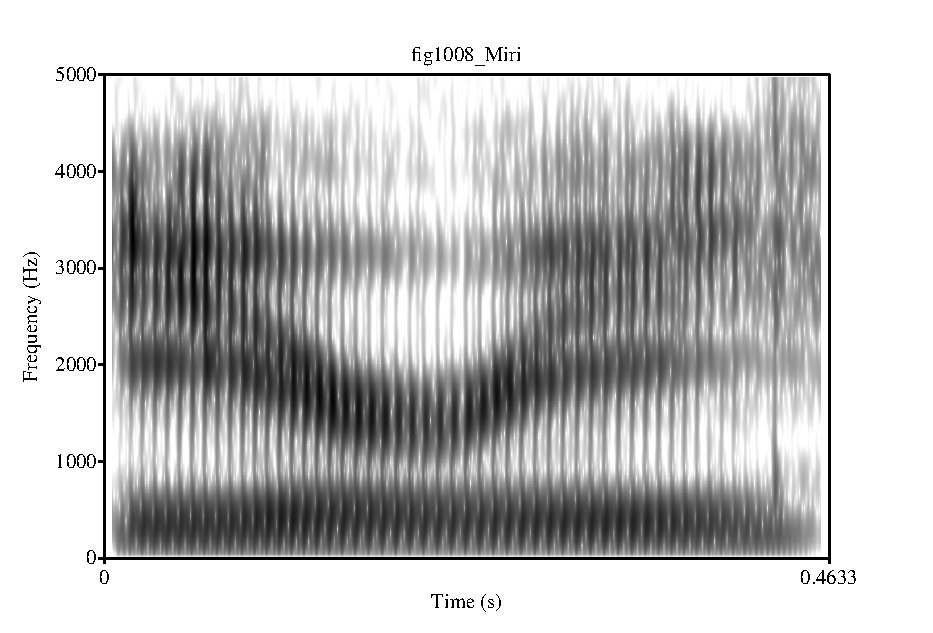
\includegraphics[width = \textwidth]{figs/iri.eps}
    \end{center}
\end{frame}

%-----------------------------------------------------------
\section*{Practice time}
%-----------------------------------------------------------

\begin{frame}{Practice Time!}
    \begin{center}
        \Huge Let's measure vowels!
    \end{center}
\end{frame}

%-----------------------------------------------------------
\section*{To Do:}
%-----------------------------------------------------------
\begin{frame}{To Do:}
    \begin{itemize}
        \item Complete the exit ticket for today on Canvas by 12:30pm.
        \item IPA Practice 1 is due Friday
        \item Quiz 3 is due Monday
        \item Lab 1 is due by Tuesday at 23:59
        \item Homework 4 is due by Tuesday at 08:30
    \end{itemize}
\end{frame}

% \subsection<presentation>*{References}
% %-----------------------------------------------------------
% \begin{frame}[t,allowframebreaks]
%   \frametitle<presentation>{References}
%     \printbibliography
% \end{frame}

\end{document}